\documentclass[thesis-en.tex]{subfiles}

\begin{document}
\section{Overview}
Based on \hyperref[sec:batsim]{Batsim}, we developed two simulators of parallel jobs with burst buffer requests. The first of them is referred to as Alloc-Only model/simulator/scheduler. It simulates allocations of compute and storage resources, computations and inter-node communication. The second - IO-Aware model - is an extension of the Alloc-Only model, which also simulates I/O network traffic. It is capable of simulating network congestion and I/O contention among running applications. The congestion of the network effectively leads to a slowdown of application runtime. 
A significant part of a simulation logic responsible for both job scheduling and simulating of burst buffer allocations lies inside a Pybatsim-based scheduler process. The remaining part which simulates computations, communication and I/O traffic is operated be the Batsim simulator process.

\section{Platform model} \label{sec:platform}
Describing a simulated supercomputer platform model capable of simulating I/O traffic requires to define many parameters such as the number of compute nodes, network topology, network bandwidth, CPU speed, burst buffer storage model and PFS model. The platform in our simulation is managed by \hyperref[sec:simgrid]{SimGrid}, which requires to be provided with a simulated platform configuration. The simplest method to achieve this is to describe a platform using SimGrid XML file format. \hyperref[sec:batsim]{Batsim} inherits and further extends this configuration format. 

\paragraph{Network topology} \label{sec:network}
SimGrid enables to use of several predefined common cluster topologies, notably:
\begin{itemize}
    \item Torus
    \item Fat-Tree
    \item Dragonfly
\end{itemize}

We decided to model the dragonfly network topology, which is a relatively novel architecture introduced in \cite{kim2008technology}. It was already deployed in Cori \cite{bhimji2016accelerating} and Piz Daint \cite{piz-daint} supercomputers. The schema of the dragonfly topology is presented in \autoref{fig:dragonfly-topology}, where squares represent routers and points represent nodes. Compute nodes in this topology are split into groups that are connected in a full graph (clique). Nodes inside a group could be arranged in various topologies such as a clique or a fat-tree. \autoref{fig:dragonfly-topology} presents a dragonfly cluster network that consists of 9 groups of nodes.

Our model inherits the SimGrid implementation of the dragonfly architecture according to \autoref{fig:dragonfly-detail}. In this model compute nodes are attached to routers, which are connected in a clique inside a chassis. Several chassis, again connected in a clique, are then forming a single group.

\autoref{lst:dragonfly} is the XML configuration of the platform used in our simulations. The tag \verb|cluster| in line 5 defines a cluster in the dragonfly topology with 108 nodes. The tag \verb|topo_parameters| specifies the topology configuration with 3 groups, 4 chassis inside a group, 3 routers per chassis and 3 nodes attached to each router. \verb|topo_parameters| is also explained in \autoref{fig:dragonfly-detail}. As shown in this figure, there could be defined several network links between different cluster components. For simplification in our configuration, there is always a single link.

% \autoref{fig:dragonfly-topology} presents a schema of a Dragonfly cluster network that consists of 9 groups of nodes. All the groups are directly connected with each other. For simplification chassis, also known as cabinets, are not shown within groups in this figure. The detailed description of the Dragonfly group is illustrated in \autoref{fig:dragonfly-detail}.

\begin{figure}[p]
    \centering
    \includesvg[width=0.6\textwidth]{images/Dragonfly-topology}
    \captionsource{Simplified overview of a Dragonfly network topology}
    {\url{https://commons.wikimedia.org/wiki/File:Dragonfly-topology.svg}}
    \label{fig:dragonfly-topology}
\end{figure}

\begin{figure}[p]
    \centering
    \includesvg[inkscapelatex=false,width=\textwidth]{images/cluster_dragonfly}
    \captionsource{Detailed overview of a Dragonfly group definition according to SimGrid}
    {\url{https://framagit.org/simgrid/simgrid/-/blob/master/examples/platforms/cluster_dragonfly.svg}}
    \label{fig:dragonfly-detail}
\end{figure}

% \begin{figure}
%     \centering
%     \includesvg[]{images/Dragonfly-topology}
%     \captionsource{Simplified overview of a Dragonfly network topology.}
%     {\url{https://commons.wikimedia.org/wiki/File:Dragonfly-topology.svg}}
%     \label{fig:dragonfly-topology}
%     % height=\measurepage doesn't work correctly
    
%     % \bigskip
%     \vspace*{\floatsep}
    
%     \includesvg[inkscapelatex=false,width=\textwidth]{images/cluster_dragonfly}
%     \captionsource{Detailed overview of a Dragonfly group definition according to SimGrid.}
%     {\url{https://framagit.org/simgrid/simgrid/-/blob/master/examples/platforms/cluster_dragonfly.svg}}
%     \label{fig:dragonfly-detail}
% \end{figure}

\begin{listing}
    \inputminted[linenos,frame=lines,style=borland]{xml}{code/dragonfly96-thesis.xml}
    \caption{XML configuration of the simulated platform}
    \label{lst:dragonfly}
\end{listing}

\paragraph{Compute and storage nodes} \label{sec:nodes}
Our cluster model consists of 108 nodes. However, only 96 of them are compute nodes. The other 12 nodes are assigned a storage role and simulate dedicated nodes for burst buffers. To be specific, \textbf{a single node in every chassis is dedicated to being a burst buffer node}, which in our cluster model means that there are 8 compute nodes per every burst buffer node. This type of shared burst buffer architecture closely resembles the architecture of Fugaku supercomputer, where one of every 16 compute nodes contains SSDs for burst buffers \cite{fugaku}.

Although 96 compute nodes is not a representative number for a modern supercomputing cluster, we decided to choose this number to make the execution traces possible to be analyses in detail during the development and fine-tuning of the simulator parameters. The described burst buffer nodes configuration is not represented in \autoref{lst:dragonfly} but specified in a Batsim simulator run command.

Another important burst buffer model assumption is no exclusiveness of storage resources for compute nodes. That is every compute node could be allocated with burst buffer located on any storage node in the platform. The performance degradation of placing burst buffer away from a compute node will be taken into account by our IO-Aware simulator. However, when allocating compute and storage resources, a scheduler attempts to find free space for a burst buffer as close as possible to allocated compute nodes according to the cluster topology.

There are also two special nodes in the platform configuration described by tags:\\ \verb|<host id="master" speed="0">| and \verb|<host id="pfs" speed="0">| (lines 12, 18). The master node is unique and is mandatory for running simulation with Batsim. It is not exposed to the scheduler process and cannot be assigned to any job. In our modes, PFS is represented in the platform by a single storage node. There is also a single network link with shared bandwidth from the computing cluster to the pfs node. I/O nodes that usually conduct I/O traffic between a supercomputer and PFS are omitted in this model.

\paragraph{Network bandwidth}
Two networks could be distinguished in the platform model:
\begin{itemize}
    \item the main compute network,
    \item the I/O network.
\end{itemize}
The main compute network simulates fabrics within the cluster that is between compute nodes and burst buffer storage nodes. We set the bandwidth of a connection to 10 Gbit/s (line 8, \verb|bw="1250MBps"|). The model of burst buffer request size, described in \autoref{sec:bbrequest}, was collected on the heterogeneous MetaCentrum grid \cite{metacentrum}. The computing grid is a collection of multiple clusters with a wide range of interconnects:
\begin{itemize}
    \item Ethernet 1 Gbit/s
    \item Ethernet 10 Gbit/s
    \item InfiniBand QDR 8 Gbit/s	
    \item InfiniBand FDR 14 Gbit/s
\end{itemize}
Furthermore, the number of links in a connection is multiplied from 1 to 4 depending on a concrete cluster, which effectively gives a range of bandwidth from 1 Gbit/s to 56 Gbit/s. The value of 10 Gbit/s lies within this range and is also small enough to make MPI-like communication and I/O traffic contention relevant.

The I/O network is a single link that connects computing cluster to the PFS. When modelling the bandwidth of this link, we wanted to capture a realistic performance of PFS as well as make the effect of I/O traffic contention emphasised enough for network congestion to have a noticeable impact on jobs runtime. The list IO500 \cite{io500} provides benchmark results of the most efficient parallel file systems. We investigated the IO500 list and found out that the performance of clusters with 96 nodes varies from 2.8 GiB/s to 9.71 GiB/s, cluster with 100 nodes represented performance from 12.68 GiB/s to 22.77 GiB/s. In general, the list shows an extensive distribution of I/O systems performance. Clusters with the number of nodes from 32 to 128 have benchmark results ranging from 0.26 GiB/s to 368.44 GiB/s. Therefore, we chose the value of 5 GB/s (line 25, \verb|bandwidth="5000MBps"|) for the shared bandwidth of our PFS model. With this value of bandwidth, I/O congestion could be observed when several I/O intensive jobs are simultaneously executed.

Other network parameters, such as latency have lesser salience in our simulation. There were derived from exemplary SimGrid configurations.

\paragraph{Burst buffer capacity}
In order for the scheduling to be both limited by compute as well as storage resources, we
assume that the total burst buffer storage in the platform should be fully utilised when all compute resources are utilised. Based on this assumption, the capacity of a burst buffer node could be estimated. In \autoref{sec:bbrequest}, we derived a model of burst buffer request size per processor. In the context of our simulation, a processor is equivalent to a compute node. The mean the obtained burst buffer request size distribution is 4.58 GiB. As mentioned in \autoref{sec:nodes}, there are 8 compute nodes per every burst buffer node. Therefore, the expected capacity of a burst buffer node should be equal to:
\[ 8 \cdot 4.58\ \text{GiB} = 36.64\ \text{GiB} = 39.34\ \text{GB} \]
Finally, we round out this value to 40 GB. Although 40 GB is not a realistic capacity for any modern SSD, this value balances job scheduling well enough between compute resources and storage resources.

However, this estimation has one downside, which comes from another assumption in our model. We assume that burst buffer space for a given compute node cannot be partitioned between burst buffer nodes. This assumption may lead to underutilisation of burst buffer storage when all compute resources are in use.

\paragraph{Remaining parameters}
The CPU speed is set to 1 Gf (line 8, \verb|speed="1Gf"|). The CPU speed does not impact a simulation as it is only used to convert runtimes from workload log to the number of FLOPS which is an input for the simulator.

Another parameter \verb|loopback_bw="1000MBps"| (line 9) is the bandwidth of a loopback link of a node. This value was left as default from exemplary configurations.

\section{Workload model} \label{sec:workload}
To perform experiments on a realistic workload, we decided to transform one of the workloads from the \href{https://www.cs.huji.ac.il/labs/parallel/workload/}{Parallel Workload Achieve} into the Batsim input format. We selected the KTH-SP2-1996-2.1-cln log as it was recorded on a cluster with 100 nodes, which is the closest number to the size of our simulated cluster from all the available logs. 

This workload log was gathered over 11 months and contains 28475 job entries. The jobs that request more than 96 compute nodes in the original log were simply discarded from our final workload. After transforming there are 28453 jobs left for execution in the simulation. 

As we developed two versions of the simulation, there are also two versions of a workload. For both versions, all submission times and walltimes of jobs were preserved according to the original log. Runtimes, however, were adjusted for the IO-Aware simulator as additional IO-phases were added to jobs.

\section{Job model} \label{sec:job}
As described in \autoref{sec:algorithms}, we consider only parallel, non-preemptive and rigid job model. For both versions of the simulation, each job in the workload is described by the following parameters:
\begin{enumerate}
    \item Requested number of compute nodes,
    \item Submission time,
    \item Walltime,
    \item FLOPS per node,
    \item Number of bytes per node to send to every other node,
    \item Requested size of burst buffer per node.
\end{enumerate}
As described in \autoref{sec:workload}, the requested number of compute nodes, submission times and walltimes are the same for both simulators and directly derived from the original log.

\begin{figure}[htb]
\centering
\begin{tikzpicture}
\draw[thick,->] (0,0) -- (11.5,0) node[anchor=north west] {time};

\filldraw[blue!30] (2,0.5) rectangle (8,2) node[midway,text=black] {Computation \& Communication};
\draw[blue!30,pattern=crosshatch, pattern color=blue!30] (8,0.5) rectangle (10,2) node[midway,text=black] {};

\draw[dashed] (0.5,4) -- (0.5,-0.1) node[anchor=north] {submit};
\draw[dashed] (2,4) -- (2,-0.1) node[anchor=north] {start};
\draw[dashed] (8,4) -- (8,-0.1) node[anchor=north] {finish};
\draw[dashed] (10,4) -- (10,-0.1) node[anchor=north] (allocation) {allocation};
\node at (10,-0.7) {end};

% \draw[thick,<->] (0.5,2.5) -- (2,2.5) node[midway,above] {wait};
% \draw[thick,<->] (2,2.5) -- (8,2.5) node[midway,above] {run};
% \draw[thick,<->] (0.5,3.2) -- (8,3.2) node[midway,above] {turnaround};
% \draw[thick,<->] (2,3.9) -- (10,3.9) node[midway,above] {wall};

\draw[decorate,decoration={brace,amplitude=6pt}] (0.5,2.4) -- node[above=6pt] {wait} (2,2.4);
\draw[decorate,decoration={brace,amplitude=6pt}] (2,2.4) -- node[above=6pt] {run} (8,2.4);
\draw[decorate,decoration={brace,amplitude=6pt}] (0.5,3.2) -- node[above=6pt] {turnaround} (8,3.2);
\draw[decorate,decoration={brace,amplitude=6pt}] (2,4) -- node[above=6pt] {wall} (10,4);

\end{tikzpicture}
\caption{Alloc-Only job model}
\label{fig:alloc-only}
\end{figure}

\paragraph{Alloc-Only job model}
\autoref{fig:alloc-only} presents Alloc-Only job model together with several time metrics. In this model, a job consists of a single phase that simulates both computations and MPI-like communication. The blue rectangle extended with the striped area represents an allocation reserved for a job with the duration equal to a user specified walltime. When a running job reaches the end of an allocation, it is terminated by the system. Naturally, when a job finishes before a walltime, all resources associated with this job are released.

The number of computations per node was generated by multiplying runtime from the original log by CPU speed, which mean that expected job runtimes in the simulation matches runtimes of original jobs. The amount of computations to execute is drawn from an artificial distribution described below. It has been set in such a way that computations dominate the majority of jobs. For simplification of implementation, computations and communication happen in parallel.

\begin{figure}[htb]
\begin{tikzpicture}
\draw[thick,->] (0,0) -- (13.5,0) node[anchor=north west] {time};

\filldraw[orange!40] (0,0.5) rectangle (2,2) node[midway,text=black,align=center] {Stage-in};
\filldraw[blue!30] (2,0.5) rectangle (5,2) node[midway,text=black,align=center] {Computation \&\\ Communication};
\filldraw[orange!40] (5,0.5) rectangle (7,2) node[midway,text=black,align=center] {Checkpoint};
\filldraw[blue!30] (7,0.5) rectangle (10,2) node[midway,text=black,align=center] {Computation \&\\ Communication};
\filldraw[orange!40] (10,0.5) rectangle (12,2) node[midway,text=black,align=center] {Stage-out};
\draw[blue!30,pattern=crosshatch, pattern color=blue!30] (12,0.5) rectangle (13,2) node[midway,text=black] {};

\draw[dashed] (0,3.2) -- (0,-0.1) node[anchor=north] {start};
\draw[dashed] (12,3.2) -- (12,-0.1) node[anchor=north] {finish};
\draw[dashed] (13,3.2) -- (13,-0.1) node[anchor=north] {};

\draw[decorate,decoration={brace,amplitude=6pt}] (0,2.4) -- node[above=6pt] {run} (12,2.4);
\draw[decorate,decoration={brace,amplitude=6pt}] (0,3.2) -- node[above=6pt] {wall} (13,3.2);

\end{tikzpicture}
\caption{IO-Aware job model}
\label{fig:io-aware}
\end{figure}

\paragraph{IO-Aware job model}
This model, shown in \autoref{fig:io-aware}, is more complex as it also simulates I/O network traffic. Jobs are divided into a variable number of phases depending on the specified number of computations per node. The number of computation and communication phases varies from 1 to 10 and are all of equally divided for a given job. They are interleaved by I/O phases which simulate checkpointing. We chose checkpointing as a popular application of burst buffers. It is simulated by transferring data from compute nodes to assigned burst buffer nodes, during which other application activities are suspended. After the checkpoint phase is finished, checkpoint data transfer from burst buffers to PFS is triggered, and the next computation phase starts concurrently.

Furthermore, jobs begin and end with data staging phases which simulates input and output data transfers between PFS and assigned burst buffer nodes. The size of the data transfers is equal to the requested burst buffer size.

As jobs in the IO-Aware model were extended with additional I/O phases, the computations phases, derived from original runtimes, had to be shortened accordingly in order for the jobs to avoid walltime exceeding. We adjust the requested total number of computations per node with the following formula:
\[ \text{round}(CPU_{speed} \cdot \text{max}(runtime - \kappa \cdot bb / bandwidth,\ 0.05 \cdot runtime)) \]
where\\ 
$CPU_{speed}$ - processor speed in FLOPS,\\ 
$runtime$ - runtime of a job from the original KTH workload log,\\
$\kappa$ - empirically found factor,\\
$bb$ - requested size of burst buffer per compute node,\\
$bandwidth$ - bandwidth of the main compute network.

We were searching for the value of the $\kappa$ parameter by generating IO-Aware workloads, running a simulation with standard backfilling scheduling and comparing results to those obtained from Alloc-Only simulation. We found that $\kappa=40$ raises similar results in terms of mean job runtimes, number of timeout jobs and waiting queue characteristics. 

We also set an upper bound for the proportion of I/O time to computation time, that is an application could spend up to 95\% of the time in I/O phases. Lastly, very short jobs, those with up to 120 seconds runtime, are assigned with a constant minimal burst buffer request size as they are most likely to timeout.

\paragraph{Network traffic model}
As the amount of network traffic is not included in Standard Workload Format, we could either omit application inter-node communication from simulation or obtain these requirements from other sources. We decided to include inter-node communication in the simulations as we find that interfering between MPI-like traffic and I/O traffic creates a more realistic simulation model. As inter-node communication is not an essential factor in our simulation, we used a normal distribution with $\mu=100\ \text{MB}$ and $\sigma=20\%$ to model the amount of network traffic of a job sent between each processor. That is, for a drawn value $\theta$, in each communication phase, each processor sends $\theta$ bytes to every other processor. It is essentially the N-N communication model. The overall application traffic is proportional to the square of the number of processors and grows linearly with the number of communication phases.

\section{Burst buffer request model} \label{sec:bbrequest}
As burst buffers are a relatively new technology, there has not been put many studies into them. Notably, the topic of burst buffer aware scheduling has been not well exploited in research. The consequence of the current state of research is a lack of available workload traces and logs that contain data about burst buffers, or models of burst buffer requests. For instance, none of the workloads in the Parallel Workloads Archive contains information about burst buffers. Furthermore, the Standard Workload Format in the latest version 2.2 does not specify a field for burst buffers.

This issue was tackled by Fan \textit{et al.} \cite{10.1145/3307681.3325401} for evaluation of their multi-resource scheduling scheme named BBSched, where two different traces and methods were used. The first trace is a four months long SLURM log collected from the Cori system \cite{cori}. Cori is a supercomputer equipped with burst buffers, so consequently, this log contains real burst buffer requests from users. Unfortunately, this log is not publicly available. The second trace is half-year Darshan log from the Theta system \cite{theta} that provides information about recorded I/O. The Theta system was not deployed at the time with any shared burst buffer. The potential burst buffer requests were estimated by the amount of data moved between PFS and nodes.

Darshan is an HPC I/O characterisation tool, and it is a part of the CODES project (described in \autoref{sec:batsim}). It is a fairly popular data source for I/O workload in HPC research related to storage and burst buffers. Exemplary papers that utilised Darshan I/O logs are \cite{6232369,10.1145/2832087.2832091}.

Another approach to I/O workload modelling was applied in \cite{8752797}. Lackner \textit{et al.} extended an existing HPC workload model with information about the amount of requested burst buffer storage capacity, stage-in and stage-out data, and the amount of intermediate data written to and read from burst buffers at runtime.

We propose yet another approach to estimate burst buffer requests. \emph{Under the assumption that a burst buffer request size is equal to the main memory request size}, we create a model of burst buffer requests based on the METACENTRUM-2013-3 workload log from the Parallel Workload Achieve. As described in \autoref{sec:workload}, we use the KTH-SP2-1996-2.1-cln log to generate the Batsim workload as it the best matches our targeted platform. However, it does not contain information on requested memory sizes. Hence, we had to use another log to obtain those information.

From the METACENTRUM-2013-3 log, we extract the data about processors requests, memory requests and execution time of each job. Then we analyse a correlation between processors requests and memory requests. Finally, we perform a fit of existing probability distributions to empirical data and test the quality of obtained models. Such a model can be later used to generate burst buffer requests for jobs in other logs. 

\paragraph{Analysis of a memory request size}
We start with loading the METACENTRUM-2013-3.swf file directly into the Pandas \cite{reback2020pandas, mckinney-proc-scipy-2010} DataFrame, which could be easily achieved with the Evalys library \cite{evalys} developed as the Batsim supplementary analysis tool. The Metacentrum log contains 5731099 jobs. We filter out jobs that do not contain information about requested memory (marked as -1) or specify requested memory to 0. After this filtering, there are 5722091 jobs left in the log. This number will be referred to as \emph{all jobs} in the text below. All the remaining jobs have the number of requested processors greater than 0.

\begin{figure}[htb]
    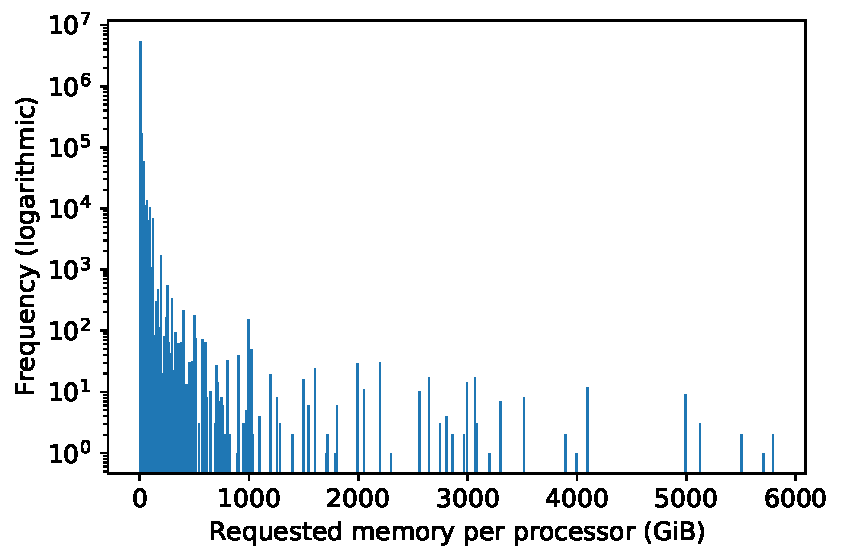
\includegraphics[width=\textwidth]{images/memory_requests_histogram.pdf}
    \caption{Histogram of memory requests of all jobs from the METACENTRUM-2013-3 log.}
    \label{fig:mem-req-hist}
\end{figure}

\begin{figure}[htb]
    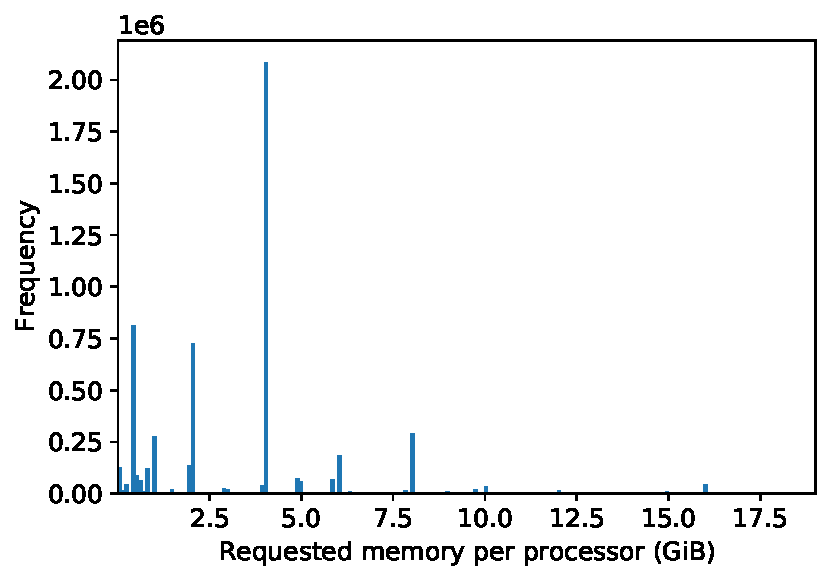
\includegraphics[width=\textwidth]{images/truncated_memory_requests_histogram.pdf}
    \caption{Histogram of memory requests from the METACENTRUM-2013-3 log with a truncated tail.}
    \label{fig:trun-mem-req-hist}
\end{figure}

% \begin{figure}
%   \begin{subfigure}[b]{0.5\textwidth}
%     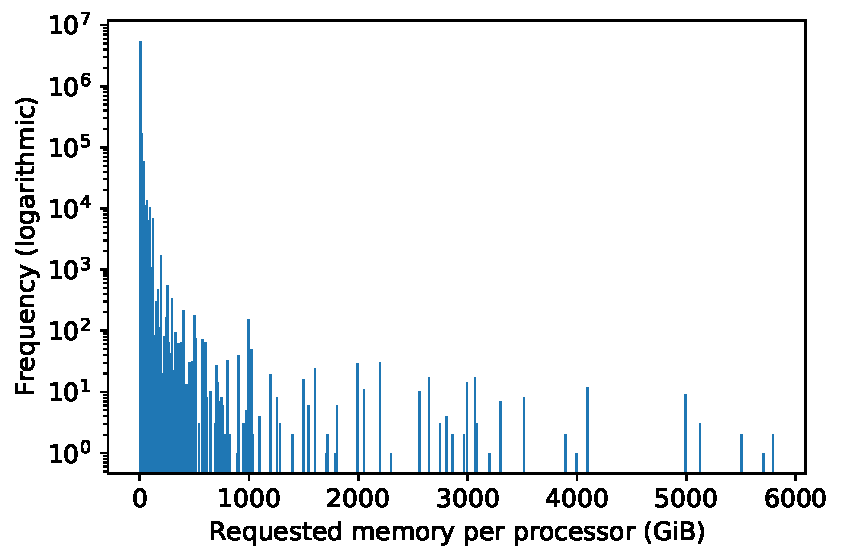
\includegraphics[width=\textwidth]{images/memory_requests_histogram.pdf}
%     \caption{Picture 1}
%     \label{fig:1}
%   \end{subfigure}
%   \hfill
%   \begin{subfigure}[b]{0.5\textwidth}
%     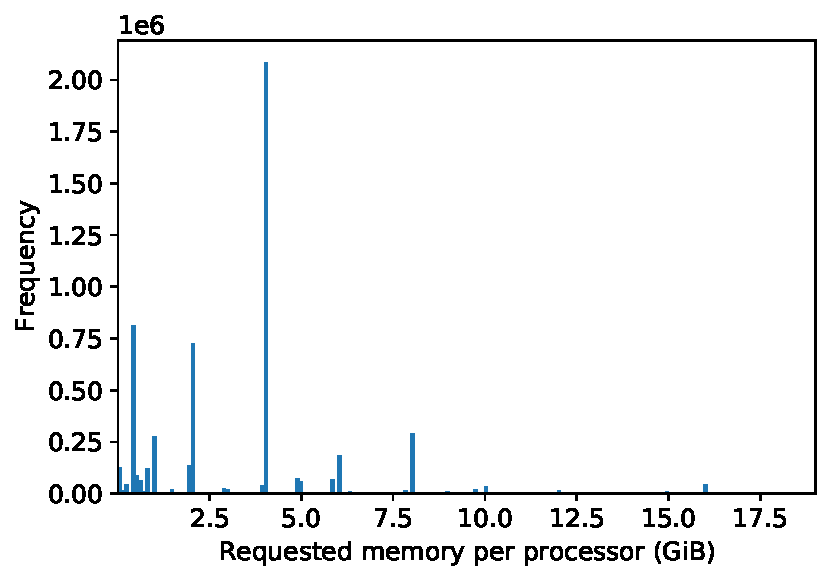
\includegraphics[width=\textwidth]{images/truncated_memory_requests_histogram.pdf}
%     \caption{Picture 2}
%     \label{fig:2}
%   \end{subfigure}
% \end{figure}

Figures \ref{fig:mem-req-hist} and \ref{fig:trun-mem-req-hist} present histograms of memory requests of jobs. In \autoref{fig:mem-req-hist}, we can observe an exponential shape of the empirical distribution with a long tail. \autoref{fig:trun-mem-req-hist} depicts a histogram with a truncated tail to the value of $2*10^7$ kilobytes. The intriguing part to notice there is a significant peak of a count of jobs requesting memory of size around 4 GB. In particular, this peak corresponds precisely to the value of 4 GiB (4294967296 bytes). We calculated that $36.444\%$ (2085360/5722091) of all jobs request 4 GiB of memory per processor. This phenomenon could be easily explained with a hypothesis that 4 GiB was a default size of memory per processor assigned to a job. All jobs which did not have explicitly specified the amount of memory were assigned with the above value.

\paragraph{Cross-correlation between requested memory size and the number of processors}
Following the guides of Dror G. Feitelson outlined in chapter 6. of \textit{Workload Modeling for Computer Systems Performance Evaluation} \cite{10.5555/2808941} there often exists several types of correlations between different attributes in computer workloads, namely:
\begin{itemize}
\item Temporal locality,
\item Spatial locality,
\item Cross-correlation among distinct workload attributes,
\item Self-similarity,
\item Long-range dependence.
\end{itemize}
In our analysis, we wanted to examine whether there exists a cross-correlation between the requested number of processors and memory per processor. If such a correlation exists, it is appropriate to model a distribution of memory as either a conditional probability distribution or a joint probability distribution with the number of processors.

\begin{figure}[htb!]
    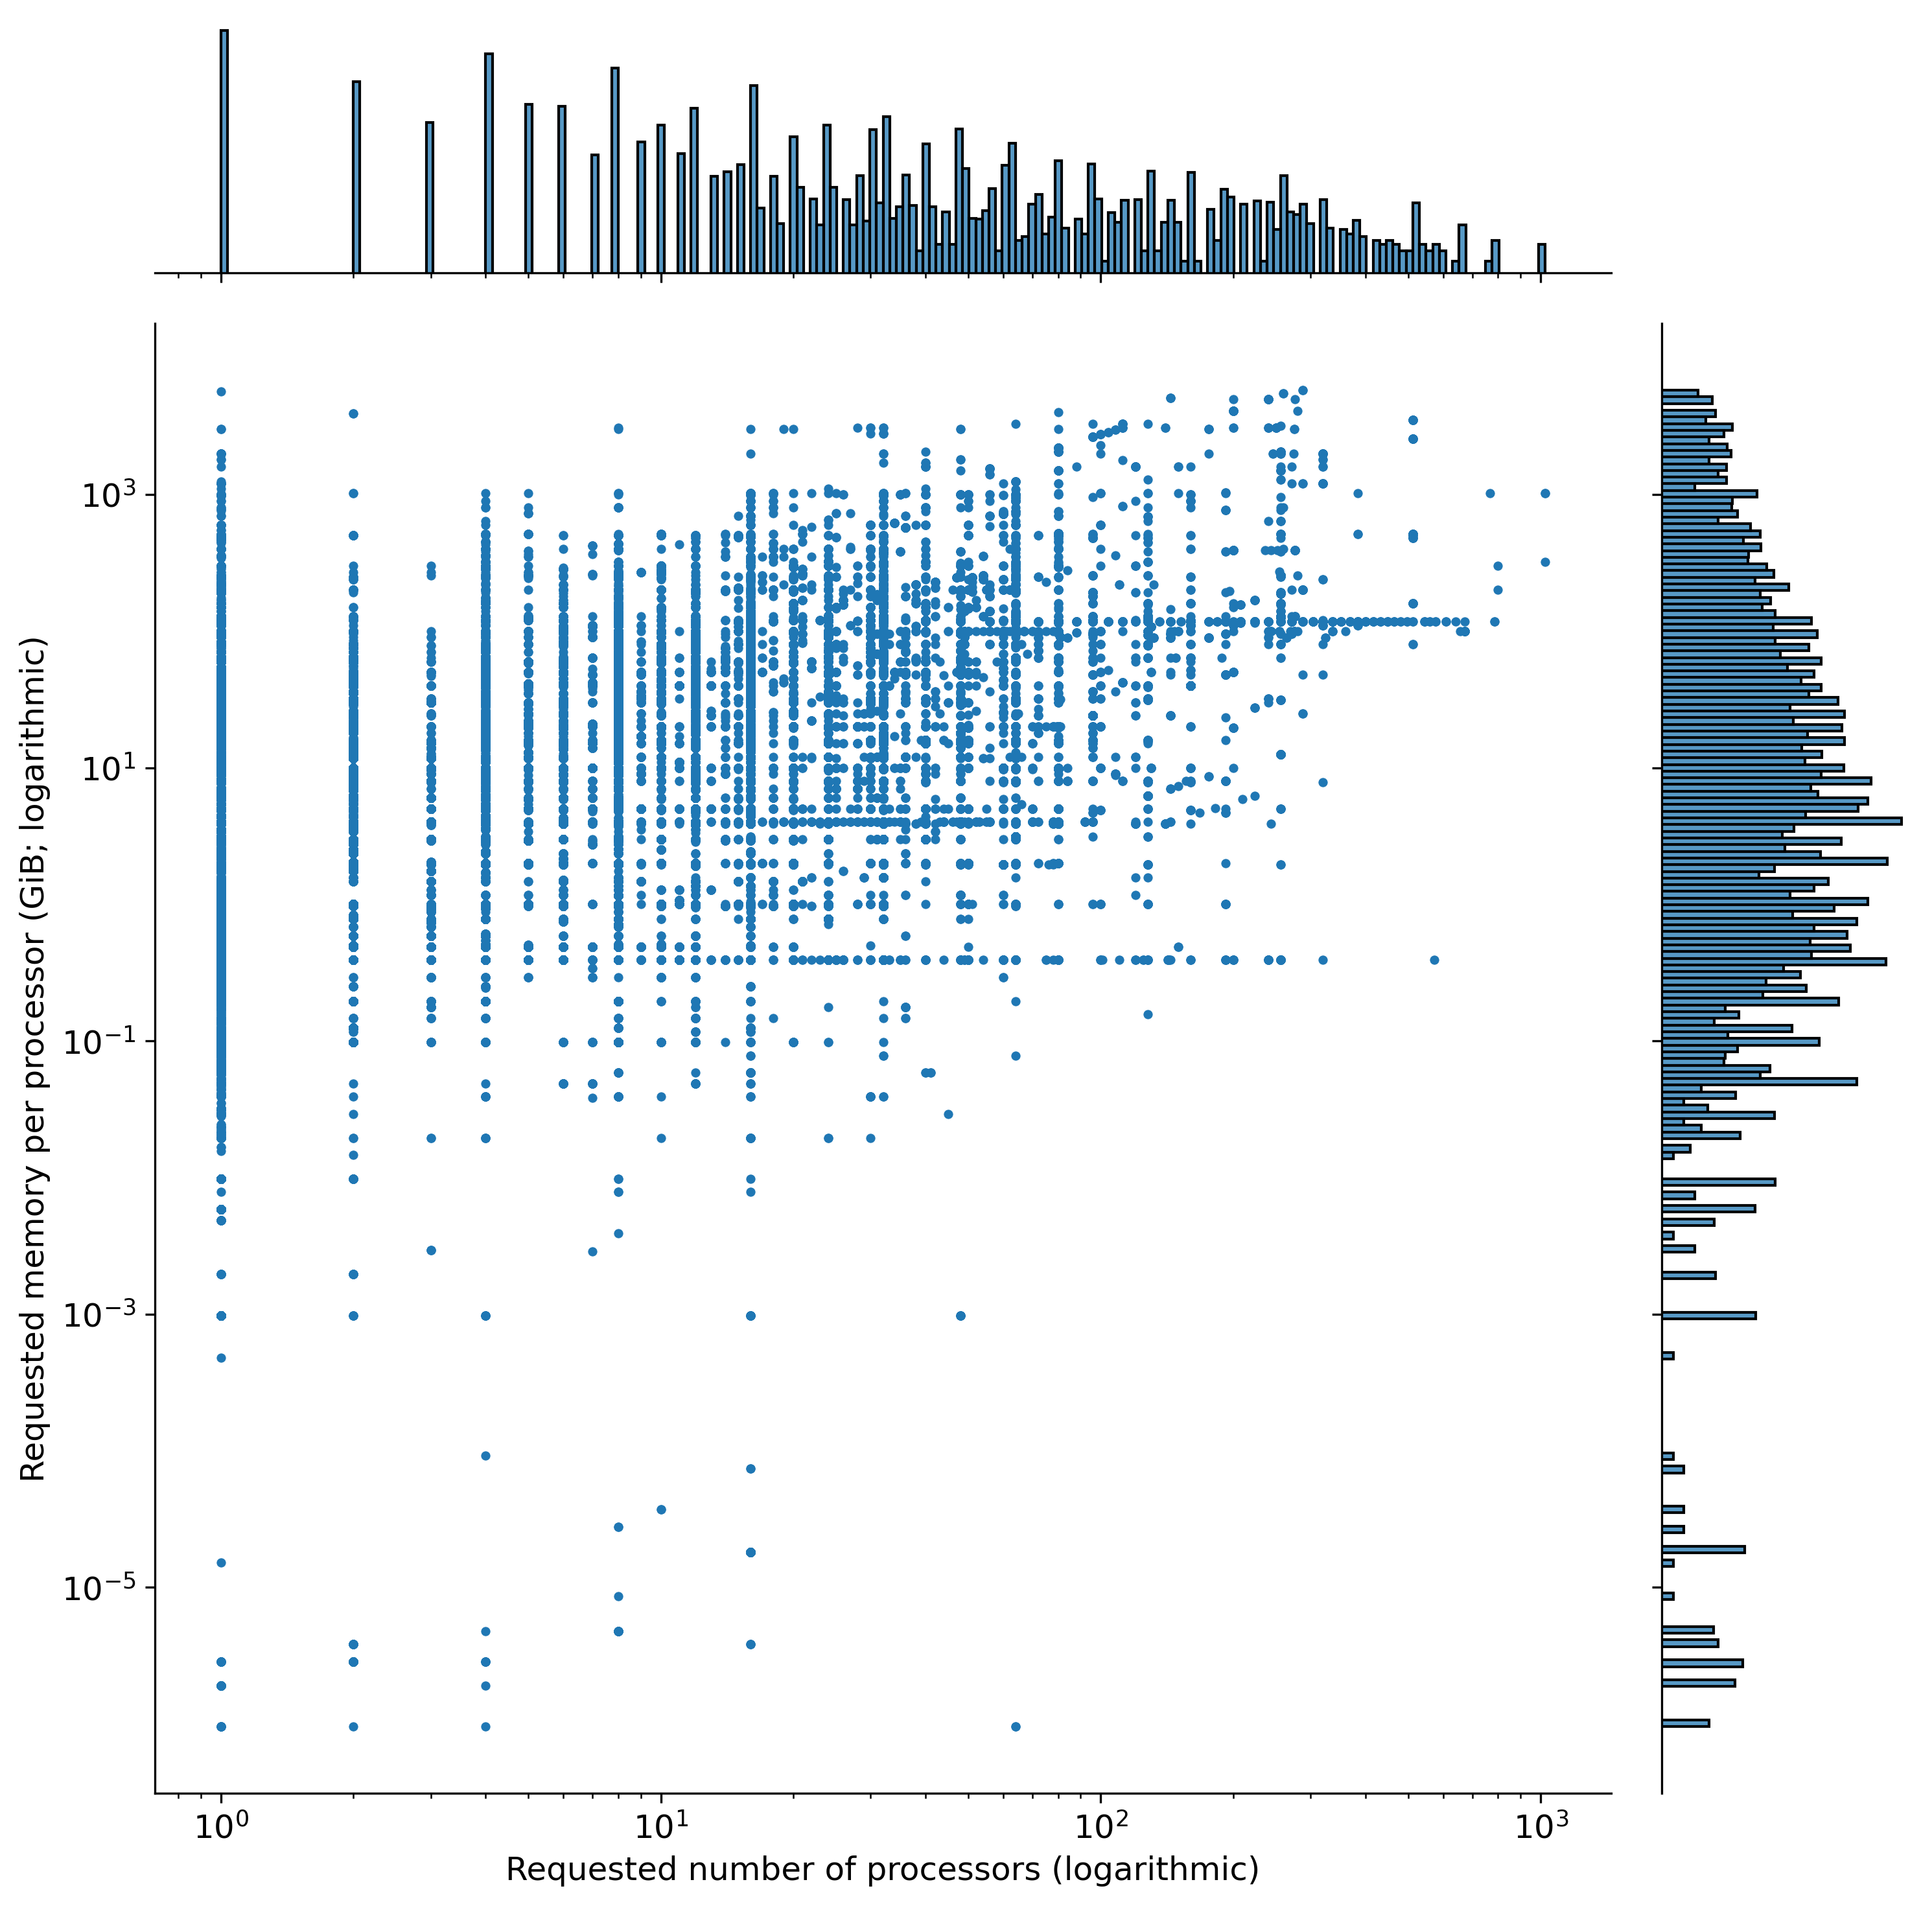
\includegraphics[width=\textwidth]{images/scatterplot.png}
    \caption{Scatterplot of joint distributions of requested number of processors and memory per processor with their related marginal distributions.}
    \label{fig:scatter}
\end{figure}

Two visual methods of investigating cross-correlations described in \cite{10.5555/2808941} are plotting a 2D surface of a joint distribution of attributes and creating a scatterplot with associated marginal distributions as in \autoref{fig:scatter}. Based on the data points in this scatterplot, it is hard to conclude the existence of a cross-correlation. However, it is visible that the majority of the jobs are concentrated on a small number of requested processors and a small amount of memory. Nonetheless, there are some significant outliers in the data set.

\begin{figure}[htb!]
    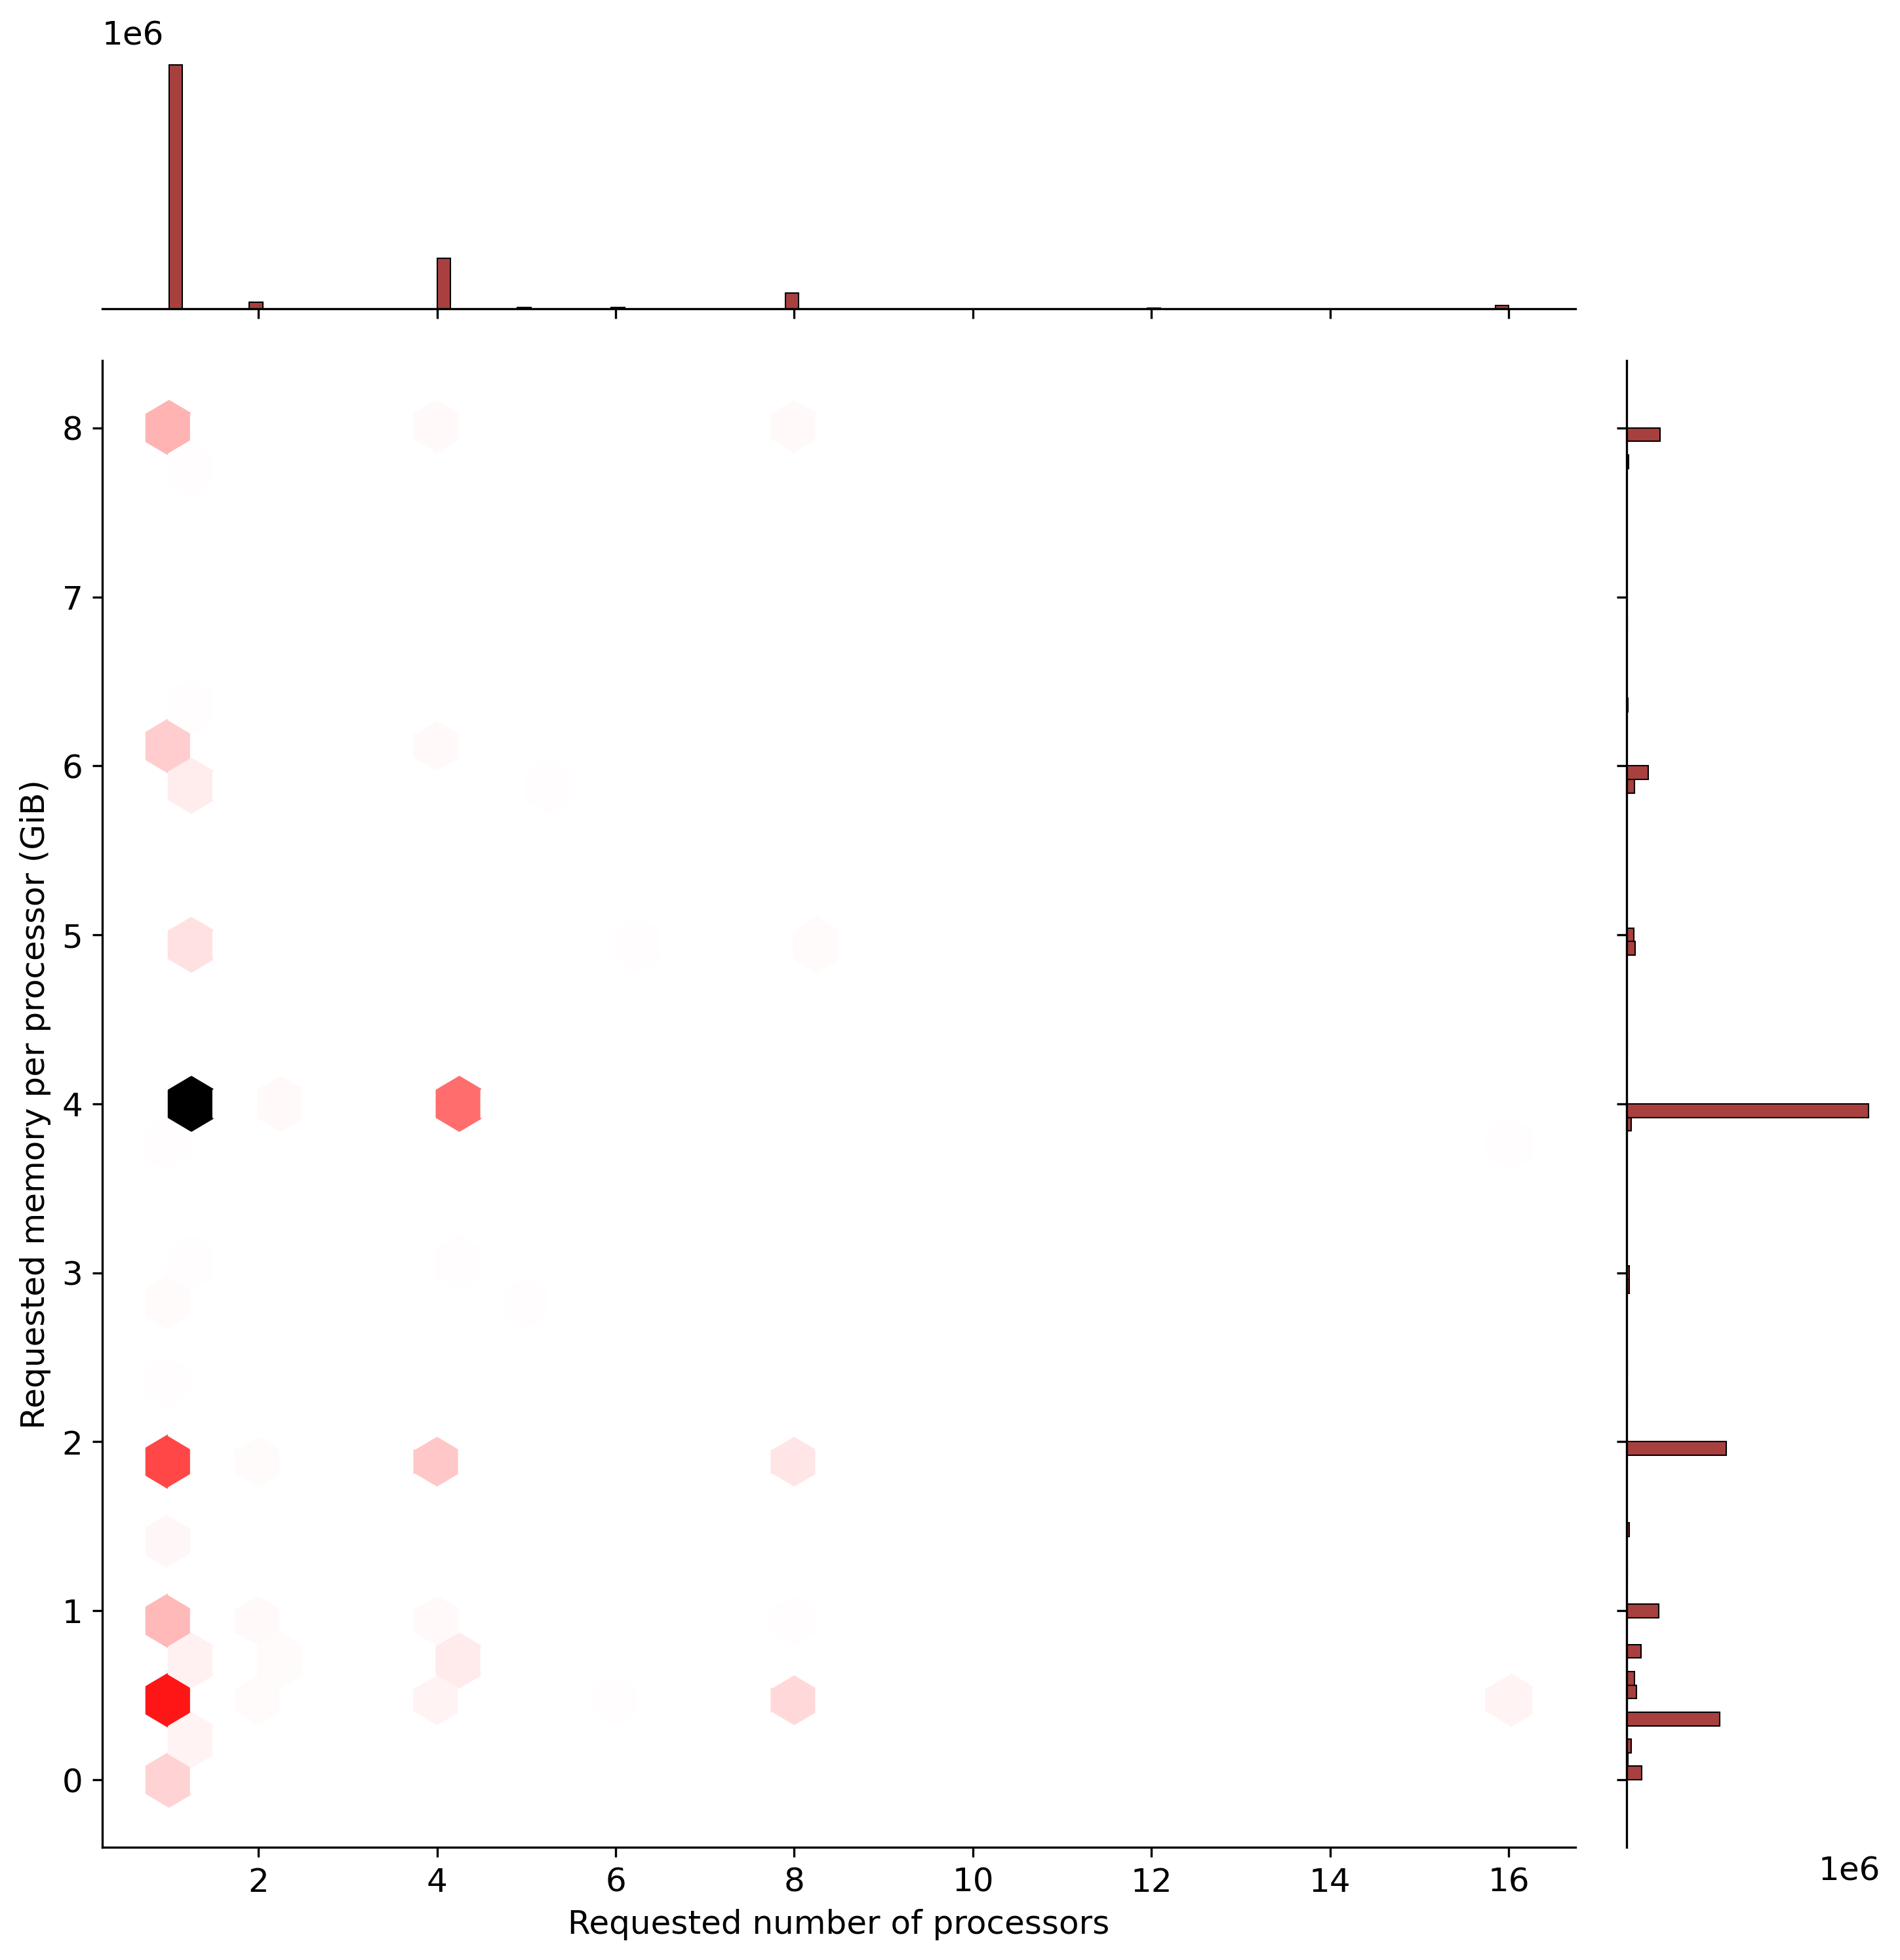
\includegraphics[width=\textwidth]{images/heatmap.png}
    \caption{Heatmap of joint distributions of the requested number of processors and memory per processor with both tails truncated. The more intense is the colour of a bin, the more frequent it is.}
    \label{fig:heatmap}
\end{figure}

\autoref{fig:heatmap} presents a heatmap of joint distributions with hexagonal bins and truncated tails of both distributions. Again there is visible a concentration of points at the value of 4 GB of requested memory. Moreover, we can observe the concentration of jobs corresponding to the powers of two of the requested number of processors.

Both of those joint distribution plots were generated with the Seaborn \cite{michael_waskom_2017_883859} Python library.

\begin{table}[h]
\centering
\begin{tabular}{ |c|c|c| } 
 \hline
 Pearson & Kendall & Spearman \\ 
 \hline
 0.345 & 0.073 & 0.088 \\ 
 \hline
\end{tabular}
\caption{Cross-correlation coefficients values between the requested number of processors and memory per processor}
\label{table:correlation}
\end{table}

As visual methods did not  indicate any confident cross-correlation, we computed correlation coefficients. \autoref{table:correlation} presents the results of Pearson, Kendall and Spearman correlation coefficients. The Pearson correlation is used to measure the quality of linear correlation in data. Our value of the Pearson coefficient indicates a very weak correlation. The downside of the Pearson coefficient is its sensitivity on outliers, which is a case in this workload. The Kendall and Spearman coefficient are not so sensible to outliers and are capable of detecting non-linear correlations. Our computed values of these coefficients indicate that there is no cross-correlation.

\begin{figure}[p]
    \centering
    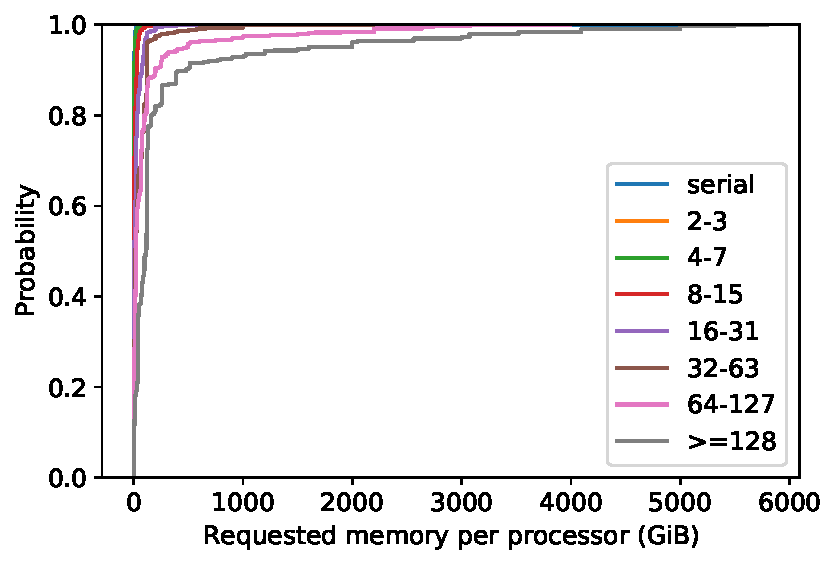
\includegraphics[width=0.95\textwidth]{images/cdf_ranges_many.pdf}
    \caption{Empirical distribution function of requested memory divided into ranges by powers of two of the number of requested processors}
    \label{fig:cdf-ranges-many}
\end{figure}

\begin{figure}[p]
    \centering
    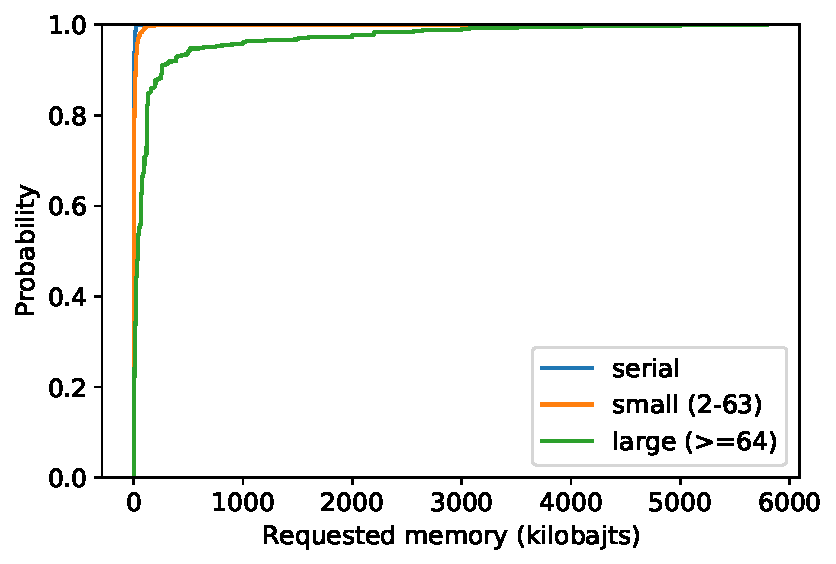
\includegraphics[width=0.95\textwidth]{images/cdf_ranges_few.pdf}
    \caption{Empirical distribution function of requested memory divided into serial, small and large jobs by the number of requested processors}
    \label{fig:cdf-ranges-few}
\end{figure}

It may also be possible that cross-correlation does not  exist in the whole data set, but only in some range of values. This hypothesis could be investigated by plotting empirical cumulative distribution functions (ECDF) of memory requests conditioned by ranges of numbers of processors. \autoref{fig:cdf-ranges-many} shows these distributions divided into ranges by powers of two of the requested number of processors. In this plot, we can observe that ECDFs of serial jobs and small jobs up to the size of 63 processors are relatively similar. The ECDF of jobs of size 64-127 is slightly different. A significant difference is visible in the shape of the ECDF of large jobs with the number of processors equal and above 128. We emphasise these difference in \autoref{fig:cdf-ranges-few}. The shapes of ECDFs suggests that the probability distribution of requested memory should be modelled taken into account the split into small and large jobs.

In order to finally determine the contribution of large jobs in a whole workload, we calculated the total processors time and memory time taken by large jobs. As we are dealing with rigid jobs, it is sufficient to sum over rectangles representing jobs, where one side is an execution time of a job and the second side it either the number of processors or amount of requested memory by the job. We define large jobs in the METACENTRUM-2013-3 log as those of size 64 or greater. There are only 5936 out of 5722091 of them, which is about $0.1\%$. They overall contribute to $11\%$ of processor time and $8.4\%$ memory time. Given that this contribution is relatively small, we decided to model the distribution of requested memory independently from the number of processors. We consider the different distribution of large jobs to have a negligible effect on the overall distribution of memory.

\paragraph{Probability distribution function model}
As we observed in \autoref{fig:mem-req-hist}, the empirical distribution of requested memory values tends to have an exponential characteristic. We want to find a probability distribution that best models the body part as well as the long tail of the empirical distribution. In order to do this, we use the package FITTER \cite{fitter} to match a sample of 10000 data points to all probability distribution available in the SciPy library \cite{2020SciPy-NMeth} and calculate a sum of squares error. Based on the error values, we selected five fairly popular distributions with different shapes: exponential, log-normal, logistic, half-logistic, beta.

\begin{table}[htb]
\centering
\begin{tabular}{ |c|c|c| } 
 \hline
 Distribution & KS statistic average \\ 
 \hline\hline
 Exponential & $0.2562 \pm 0.0004$ \\ 
 \hline
 Log-normal & $0.2200 \pm 0.0009$ \\ 
 \hline
 Logistic & $0.2490 \pm 0.0005$ \\ 
 \hline
 Half-logistic & $0.3047 \pm 0.0029$ \\ 
 \hline
 Beta & $0.2247 \pm 0.0082$ \\ 
 \hline
\end{tabular}
\caption{Values of Kolmogorov-Smirnov D-statistic for the fitted distributions}
\label{table:kstest}
\end{table}

We perform 5-fold cross-validation to achieve a reliable fit of distribution and test the goodness of fit. That is, we divide the data set into five parts. Then five times repeat the following procedure: leave out one of the parts as a test set and fit a probability distribution to remaining data points. On the left out part, we perform the Kolmogorov-Smirnov test for the goodness of fit. In \autoref{table:kstest} are presented the averaged results of the Kolmogorov-Smirnov test and their standard deviations. The lower is a value of the Kolmogorov-Smirnov D-statistic the better is a fit of a distribution.  We rate the quality of obtained models based on the values of the Kolmogorov-Smirnov D-statistic and standard deviations of fitted distribution parameters. These criteria guided us to the conclusion that the log-normal distribution provides the best fit to the empirical data.

\begin{figure}[p]
    \centering
    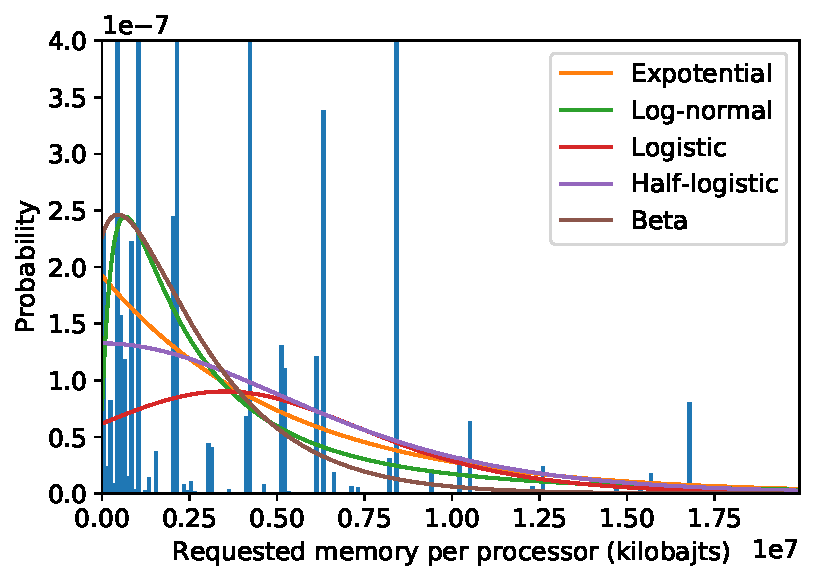
\includegraphics[width=0.95\textwidth]{images/fitted_pdfs.pdf}
    \caption{Histogram of memory requests and probability density functions of fitted distributions. Both axes of the histogram are truncated.}
    \label{fig:fitted-pdfs}
\end{figure}

\begin{figure}[p]
    \centering
    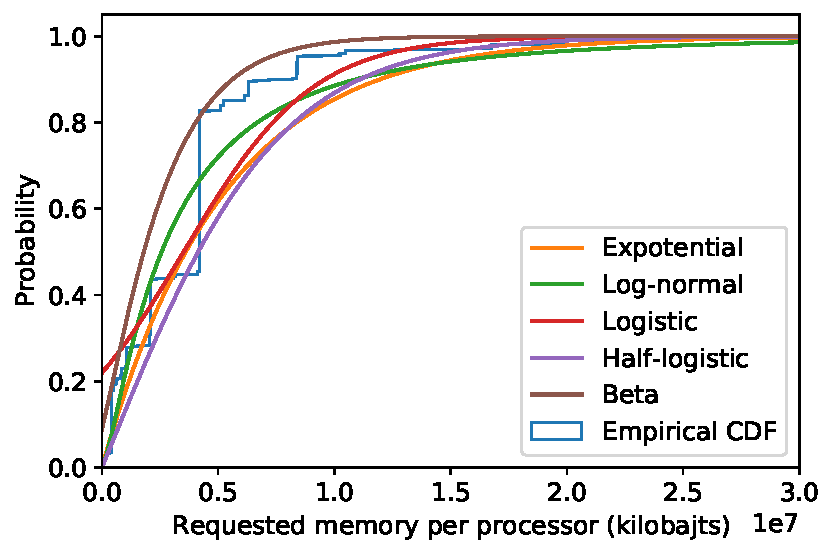
\includegraphics[width=0.95\textwidth]{images/fitted_cdfs.pdf}
    \caption{Empirical cumulative distribution function of requested memory and cumulative distribution functions of fitted distributions. The X-axis is truncated.}
    \label{fig:fitted-cdfs}
\end{figure}

Figures \ref{fig:fitted-pdfs} and \ref{fig:fitted-cdfs} show probability distribution functions and cumulative distribution functions of the five selected distributions fitted to the data. We may observe that all selected distributions except the logistic provide natural noise to the peak at 4 GiB in the data.

The general formula for the probability density function of the log-normal distribution is:
\[ f(x) = \frac{1}{\sigma x \sqrt{2\pi}} \exp\biggl( -\frac{\ln((x - \theta) / m)^2}{2\sigma^2} \biggr); \qquad x>\theta;\ \sigma>0;\ m>0 \]
where $\sigma$ is the shape parameter, $\theta$ is the location parameter and $m$ is the scale parameter.

As parameters to our distributions, we used averaged values of parameters fitted during the cross-validation. The fitted parameters for the log-normal distribution are in \autoref{table:lognorm-params}. Selected statistics of this distribution are presented in \autoref{table:lognorm-stats}.
\begin{table}[htb]
\centering
\begin{tabular}{ |c|c| } 
  \hline
  Shape $\sigma$ & 1.09725 \\ 
  \hline
  Location $\theta$ & -150361 \\ 
  \hline
  Scale $m$ & 2714115 \\ 
  \hline
\end{tabular}
\caption{Parameters of the fitted log-normal distribution.}
\label{table:lognorm-params}
\end{table}

\begin{table}[htb]
\centering
\begin{tabular}{ |c|c| } 
  \hline
  Mean & 4804884 \\ 
  \hline
  Standard deviation & 7569200 \\ 
  \hline
  Median & 2563753 \\ 
  \hline
  Approximated mode & 665852 \\ 
  \hline
\end{tabular}
\caption{Statistics of the fitted log-normal distribution in kilobytes.}
\label{table:lognorm-stats}
\end{table}

\begin{samepage}
The log-normal distribution could be directly programmatically reproduced using the SciPy library with the following lines of code:
\begin{minted}[samepage]{python}
from scipy import stats
distribution = stats.lognorm(
    s=1.09725, 
    loc=-150361, 
    scale=2714115
)
\end{minted}
\end{samepage}

\end{document}